\section{Diseño del sistema operativo propuesto}

\subsection{Diagrama de Arquitectura General de SerenityOS}

El sistema operativo \texttt{SerenityOS} tiene una arquitectura monolítica que se organiza en varias capas interconectadas. A continuación se describen los componentes clave de su estructura:

\subsubsection{Kernel}
El \texttt{Kernel} es el núcleo del sistema operativo y gestiona los recursos del hardware. Las funciones principales del kernel incluyen:
\begin{itemize}
    \item \textbf{Gestión de Procesos:} Controla la ejecución de procesos.
    \item \textbf{Gestión de Memoria:} Administra la memoria física y virtual.
    \item \textbf{Sistema de Archivos:} Facilita el acceso y almacenamiento de archivos.
    \item \textbf{Controladores de Hardware:} Permiten la interacción con dispositivos de hardware.
\end{itemize}

\subsubsection{Espacio de Usuario}
El \texttt{Espacio de Usuario} contiene las aplicaciones y herramientas que interactúan con el kernel mediante llamadas al sistema. Se compone de:
\begin{itemize}
    \item \textbf{Aplicaciones:} Programas que el usuario ejecuta.
    \item \textbf{Bibliotecas:} Funciones reutilizables que proveen servicios a las aplicaciones.
    \item \textbf{Servidor de GUI:} Gestiona la interfaz gráfica del usuario.
\end{itemize}

\subsubsection{Herramientas de Desarrollo}
Las herramientas de desarrollo permiten la creación, compilación y depuración del sistema y aplicaciones. Incluyen:
\begin{itemize}
    \item \textbf{Entorno de Desarrollo (IDE):} Facilita la programación y gestión del código fuente.
    \item \textbf{Compiladores (GCC):} Transforman el código fuente en ejecutables.
    \item \textbf{Depuradores (GDB):} Ayudan a detectar y solucionar errores en el código.
\end{itemize}

\subsubsection{Comunicación entre el Kernel y el Espacio de Usuario}
La comunicación entre el kernel y el espacio de usuario se realiza mediante \textbf{syscalls} (llamadas al sistema), que permiten a las aplicaciones acceder a los servicios del kernel de forma segura.

\subsubsection{Hardware}
El \texttt{Hardware} representa los componentes físicos del sistema (CPU, memoria, almacenamiento), con los cuales el kernel interactúa para gestionar los recursos físicos.

\begin{figure}[H]
    \centering
    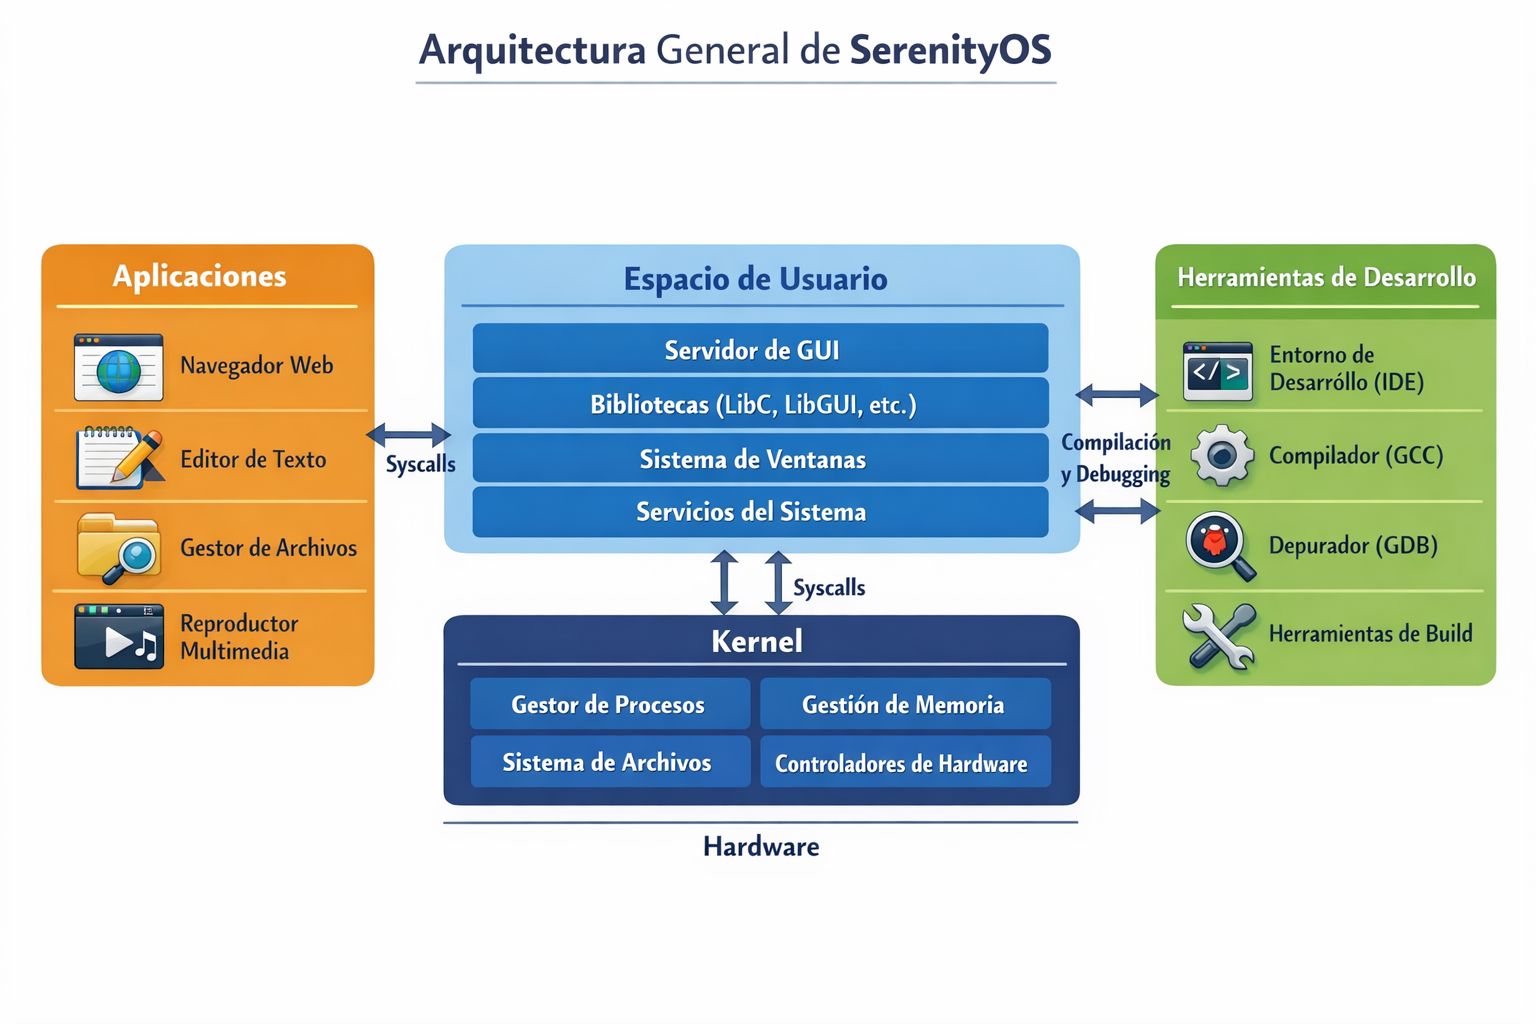
\includegraphics[width=1\linewidth]{figures/Diagrama.png}
    \caption{Diagrama de la arquitectura general de SerenityOS, mostrando las principales capas y su interacción mediante syscalls.}
    \label{fig:placeholder}
\end{figure}


\subsection{Componentes a implementar}

\subsubsection{Bootloader de SerenityOS}

El \textbf{bootloader} de **SerenityOS** se encarga de inicializar el sistema antes de que el kernel tome control. Su principal función es cargar el kernel en memoria y pasarle parámetros necesarios.

\begin{itemize}
  \item \textbf{Selección de dispositivo de arranque}: Usando el parámetro \texttt{root={value}}, se especifica el dispositivo desde el cual se va a arrancar el sistema.
  \item \textbf{Carga del Kernel}: El bootloader carga el kernel en memoria y le pasa los parámetros de configuración.
  \item \textbf{Framebuffer}: Si el bootloader proporciona un framebuffer, se configura para mostrar la salida gráfica; si no, se usa un framebuffer de texto.
\end{itemize}

\textbf{Parámetros de arranque}

Algunos parámetros clave que se pueden pasar al kernel incluyen:
\begin{itemize}
  \item \textbf{acpi}: Configura el soporte de ACPI (\texttt{on}, \texttt{limited}, \texttt{off}).
  \item \textbf{graphics\_subsystem\_mode}: Controla el modo gráfico (\texttt{on}, \texttt{off}, \texttt{limited}).
  \item \textbf{root}: Especifica el dispositivo raíz.
  \item \textbf{init}: Define el programa de inicialización que ejecutará el kernel (\texttt{SystemServer} por defecto).
\end{itemize}

\textbf{Selección de dispositivo de arranque}

Se pueden usar varias opciones de direccionamiento, como:
\begin{itemize}
  \item \texttt{block0:0}, \texttt{ata0:0:0}, \texttt{nvme0:1:0}, \texttt{lun0:0:0}.
\end{itemize}

El bootloader es esencial para preparar el sistema y controlar el arranque del kernel con las configuraciones adecuadas.


\subsubsection{Kernel Básico de SerenityOS}

El \textbf{kernel} de **SerenityOS** es el núcleo central del sistema operativo, responsable de gestionar los recursos del hardware y proporcionar servicios esenciales para el espacio de usuario. Su diseño está orientado a ser sencillo, pero eficiente, permitiendo la administración de procesos, memoria y dispositivos.

\begin{itemize}
  \item \textbf{Gestión de dispositivos}: El kernel interactúa con el hardware mediante controladores y subsistemas de dispositivos. Algunos de los controladores más importantes incluyen los relacionados con la gráfica (\texttt{GraphicsSubsystem}) y el almacenamiento (\texttt{AHCILocking}).
  \item \textbf{Interfaz de entrada/salida}: La clase \texttt{IOWindow} abstrae las operaciones específicas de la plataforma para facilitar la compilación en arquitecturas no x86. Este enfoque mejora la portabilidad del sistema a diferentes plataformas.
  \item \textbf{Sistema de archivos RAMFS}: El kernel implementa un sistema de archivos en RAM (\texttt{RAMFS}), que permite manejar archivos y directorios completamente en memoria.
  \item \textbf{Contenedores y aislamiento}: El kernel ofrece mecanismos de aislamiento mediante contenedores para ejecutar procesos de forma segura. Estos contenedores se basan en clases como \texttt{ScopedSpinLock} para gestionar los bloqueos en secciones críticas.
  \item \textbf{Interacción con el espacio de usuario}: El kernel expone datos importantes sobre los procesos y el sistema a través de \texttt{ProcFS} y \texttt{SysFS}, lo que permite que los programas del espacio de usuario interactúen con el sistema de manera eficiente.
\end{itemize}

\textbf{Componentes clave del Kernel}

\begin{itemize}
  \item \textbf{Gestión de gráficos}: El \texttt{Kernel Graphics Subsystem} gestiona todos los dispositivos gráficos, incluyendo aceleración 3D y mapeo de memoria de dispositivos gráficos.
  \item \textbf{Manejo de procesos}: El kernel gestiona los procesos mediante el uso de \texttt{ProcFS}, que proporciona información detallada sobre los procesos en ejecución.
  \item \textbf{Manejo de memoria}: La gestión de la memoria en el kernel se basa en un sistema de páginas, con soporte para asignación dinámica y manejo de fallos de página.
  \item \textbf{Interacción con hardware}: Utiliza direcciones relativas del hardware para seleccionar y acceder a dispositivos, como \texttt{nvme0:1:0} o \texttt{ata0:0:0}, para interactuar con dispositivos de almacenamiento.
\end{itemize}

El \textbf{kernel de SerenityOS} es un sistema monolítico que ofrece un enfoque directo para gestionar todos los aspectos de la máquina, desde la inicialización de dispositivos hasta la gestión de memoria y procesos. Su simplicidad y eficiencia son clave para el rendimiento del sistema operativo.



\subsubsection{Gestión de Procesos en SerenityOS}

La \textbf{gestión de procesos} en **SerenityOS** se encarga de crear, gestionar y mantener la información relevante sobre los procesos en ejecución. El kernel expone detalles sobre los procesos a través de \texttt{ProcFS} y facilita la interacción con estos procesos.

\begin{itemize}
  \item \textbf{Procesos y su gestión}: El kernel gestiona los procesos mediante el sistema de archivos \texttt{ProcFS}, el cual proporciona una interfaz para obtener información sobre los procesos en formato JSON.
  \item \textbf{ProcessManager}: En el espacio de usuario, la clase \texttt{ProcessManager} se encarga de gestionar los procesos en el sistema, incluyendo la creación, actualización y eliminación de procesos. Esta clase se utiliza en bibliotecas como \texttt{LibWebView} y está vinculada a la interfaz gráfica de usuario en aplicaciones como el navegador de SerenityOS.
  \item \textbf{Información de los procesos}: Cada proceso tiene entradas en \texttt{ProcFS} que incluyen enlaces simbólicos a su directorio de trabajo (\texttt{cwd}), su ejecutable (\texttt{exe}), sus descriptores de archivo abiertos (\texttt{fds}), y otros detalles como las pilas de ejecución (\texttt{stacks}) y las promesas de seguridad (\texttt{pledge}).
  \item \textbf{Interacción con el espacio de usuario}: Los programas del espacio de usuario interactúan con los procesos mediante el uso de \texttt{ProcFS} para obtener información sobre el estado de los procesos, como las asignaciones de memoria (\texttt{vm}) y los procesos hijos (\texttt{children}).
\end{itemize}

\textbf{Componentes clave en la gestión de procesos}

\begin{itemize}
  \item \textbf{Proceso y Sistema de Archivos \texttt{ProcFS}}: Permite exponer información de los procesos en el sistema de archivos \texttt{/proc}.
  \item \textbf{Clase \texttt{ProcessManager}}: Esta clase se encarga de administrar los procesos en el sistema, incluyendo la creación y gestión de los mismos en el espacio de usuario.
  \item \textbf{Interfaz con \texttt{ProcFS}}: Los procesos pueden ser consultados en \texttt{/proc} donde se encuentran directorios específicos por cada proceso con información detallada sobre su estado y recursos.
\end{itemize}

La \textbf{gestión de procesos} en **SerenityOS** está diseñada para ser sencilla pero eficiente, proporcionando una interfaz clara tanto para el espacio de usuario como para el kernel para gestionar y supervisar los procesos en ejecución.

\subsubsection{Gestión de Memoria en SerenityOS}

La \textbf{gestión de memoria} en **SerenityOS** es crucial para administrar los recursos de memoria del sistema, proporcionando asignación eficiente, protección y validación. El \texttt{MemoryManager} gestiona tanto la memoria física como la virtual para asegurar el funcionamiento estable del sistema.

\begin{itemize}
  \item \textbf{MemoryManager}: El \texttt{MemoryManager} es responsable de gestionar la memoria del sistema, incluida la asignación de páginas físicas y virtuales, y la protección de áreas críticas como el código del kernel.
  \item \textbf{Regiones de Memoria}: La memoria se organiza en \texttt{Regiones}, gestionadas por \texttt{RegionTree}, que permiten la asignación dinámica tanto para el kernel como para los procesos de usuario.
  \item \textbf{Protección de Memoria}: Se implementan mecanismos de protección para evitar la modificación de áreas críticas, como las secciones de solo lectura del kernel, utilizando \texttt{PageDirectory} para garantizar la seguridad.
  \item \textbf{Paginación y Manejo de Páginas}: El sistema utiliza tablas de páginas (\texttt{PageDirectory}) para mapear direcciones virtuales a físicas, gestionando la asignación de páginas y los fallos de página de manera eficiente.
  \item \textbf{Memoria Física y Virtual}: La memoria física y virtual es gestionada mediante \texttt{PhysicalMemoryRange}, mapeando direcciones físicas a direcciones virtuales para los procesos, garantizando el aislamiento de la memoria.
  \item \textbf{Asignación de Memoria y Gestión de Fallos}: Cuando ocurre un fallo de página, el \texttt{MemoryManager} asigna nuevas páginas de memoria y actualiza las tablas de páginas para garantizar el acceso adecuado a la memoria.
  \item \textbf{Comprobaciones y Validación}: El \texttt{MemoryManager} valida los accesos a la memoria, asegurándose de que los punteros de la pila y las direcciones de memoria sean correctos antes de permitir operaciones de acceso.
\end{itemize}

La gestión de memoria en **SerenityOS** asegura una asignación dinámica y eficiente, con protección de áreas críticas y validación de accesos para mantener la estabilidad y seguridad del sistema.

\subsubsection{Sistema de archivos}
\subsubsection{Interfaz de usuario (CLI mínima)}
\subsection{Políticas de planificación y manejo de recursos}
\subsection{Flujo de ejecución del sistema}
